\documentclass[conference]{IEEEtran}
\usepackage[T1]{fontenc}
\usepackage{amsmath}
\usepackage{graphicx}
\usepackage{float}
\usepackage{url}
\usepackage{booktabs}

\title{Proof of Concept: Embedded Light Classification Using Quantized KDE Surfaces}
\author{\IEEEauthorblockN{Mauricio Chacin}
\IEEEauthorblockA{Project 1 -- Proof of Concept Report\\
October 2026}}

\begin{document}
\maketitle

\begin{abstract}
This report documents a proof of concept for classifying light conditions using two sensor channels and a compact classifier intended to run on a microcontroller. The pipeline represents each observation in a two-dimensional feature space, estimates a kernel-density surface for each class, samples the surfaces on a fixed grid, quantizes the grid values to unsigned 8-bit integers, and performs embedded lookup with a rejection option for observations outside supported regions. The supplied desktop comparison contains four known classes and reports 100\% agreement between the continuous KDE reference and the stored \texttt{uint8} model over the evaluated observations (480 total). This agreement establishes consistency between the two implementations, not independently measured real-world classification accuracy. A raw-versus-filtered analysis of the 2712-sample recording shows that the filter removes most transient excursions (167 to 25 samples deviating more than 20 counts from a local median) and reduces spurious class changes (124 to 76) while leaving per-class mean levels essentially unchanged. Logged prediction time has a median of 6~$\mu$s and a 95th percentile of 8~$\mu$s, and the lookup tables occupy 1040 bytes.
\end{abstract}

\begin{IEEEkeywords}
light classification, embedded machine learning, kernel density estimation, quantization, sensor filtering, ESP32
\end{IEEEkeywords}

\section{Objective and Scope}
The objective is to demonstrate that light-related sensor measurements can be converted into a compact representation and classified on-device without requiring the full desktop model at inference time. The prototype uses a UV measurement and an infrared/light measurement as its two input channels. The intended target is an ESP32-class microcontroller; the current firmware uses a UV analog input and an I\textsuperscript{2}C light sensor.

The proof of concept evaluates four questions:
\begin{enumerate}
    \item Can the measured sensor features distinguish the four known classes in the collected dataset?
    \item Does the compact, quantized lookup model reproduce the continuous desktop KDE decisions?
    \item Does filtering suppress transient measurement glitches while preserving class-discriminating signal differences?
    \item What are the memory, latency, and runtime costs of prediction on the target device?
\end{enumerate}
Section~\ref{sec:eval} answers these questions in turn: class separation and desktop/quantized agreement, filter justification from the recorded signal, and prediction cost from the device log. Where a quantity was derived analytically rather than measured, the text says so.

\section{Classification Pipeline}
\subsection{Input features and preprocessing}
Each observation is represented by a two-dimensional vector
\begin{equation}
    \mathbf{x} = [u, r],
\end{equation}
where $u$ is the UV sensor feature and $r$ is the infrared/light sensor feature. The firmware and desktop preprocessing must apply the same transformation and scaling bounds; otherwise, the embedded lookup may address a different grid cell than the desktop model.

The current firmware configuration includes an exponential moving average (EMA) coefficient of $\alpha=0.2$. For a raw sample $x_t$, the filtered value is
\begin{equation}
    y_t = \alpha x_t + (1-\alpha)y_{t-1}.
\end{equation}
Section~\ref{sec:filter} justifies this setting using the recorded signal. The logged \texttt{ir} column reproduces this recursion to within 0.01 counts (the logging resolution) when seeded with the first logged raw value, which confirms the coefficient and the filter order (filter first, then feature mapping). Because \texttt{rawUV} is identically zero in the recording, the UV channel's filtering cannot be verified from these data, and the in-recording evidence below concerns the IR channel only.

\subsection{Continuous KDE reference}
A separate kernel density estimate is constructed for each known class. Given class $c$, training samples $\mathbf{x}_{c,i}$, and bandwidth $h$, the estimated density is represented generally as
\begin{equation}
    \hat f_c(\mathbf{x}) =
    \frac{1}{N_c h^d}\sum_{i=1}^{N_c}
    K\!\left(\frac{\mathbf{x}-\mathbf{x}_{c,i}}{h}\right),
\end{equation}
where $d=2$ and $K$ is the kernel used by the implementation. The class score is obtained from the corresponding density surface. 
Figure~\ref{fig:continuous} shows the supplied continuous per-class surfaces. These surfaces visualize where the training data support each class and help reveal overlap or unsupported regions.

\begin{figure}[H]
    \centering
    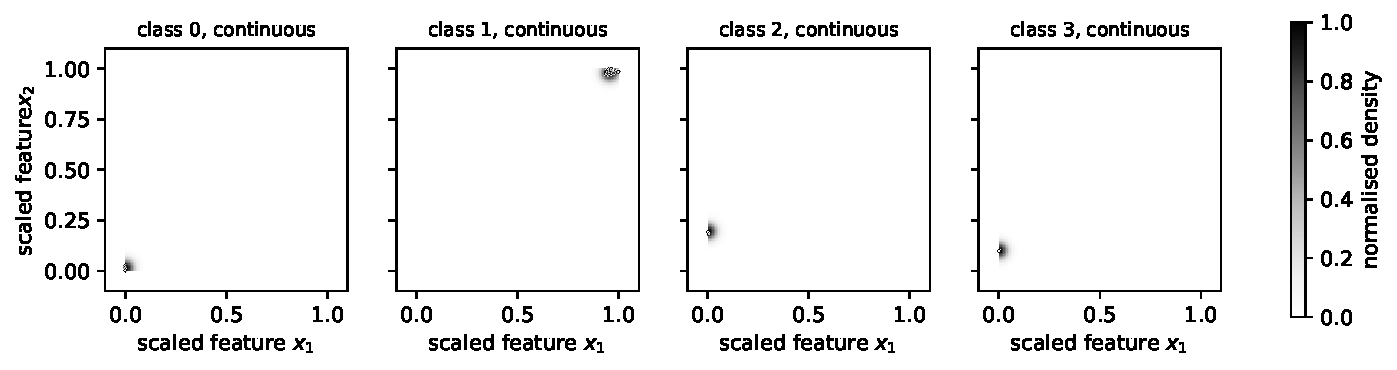
\includegraphics[width=\linewidth]{class_surfaces_continuousLight.pdf}
    \caption{Continuous per-class KDE surfaces for the light-classification dataset.}
    \label{fig:continuous}
\end{figure}

\subsection{Grid quantization and embedded inference}
The continuous surfaces are sampled onto a $G\times G$ grid and quantized to \texttt{uint8}. At inference time, the feature vector is scaled using the saved bounds, mapped to a grid location, and looked up in the stored class surfaces. A rejection threshold $\tau$ is used to return \emph{unknown} when no class has sufficient support. The grid is a compact approximation of the desktop decision surfaces; it is not a retrained model.

For $K=4$ classes and $G=16$, the class tables require
\begin{equation}
    M_{\mathrm{table}} = K G^2 = 4(16^2)=1024\ \text{bytes}.
\end{equation}
Four 32-bit scaling bounds require a further $4\times4=16$ bytes, giving 1040 bytes for these two data structures. This excludes class-name strings, constants, alignment, program code, stack, sensor libraries, and other firmware state. The precise compiled flash/RAM footprint must be measured on the target rather than estimated from table size alone.

\begin{figure}[H]
    \centering
    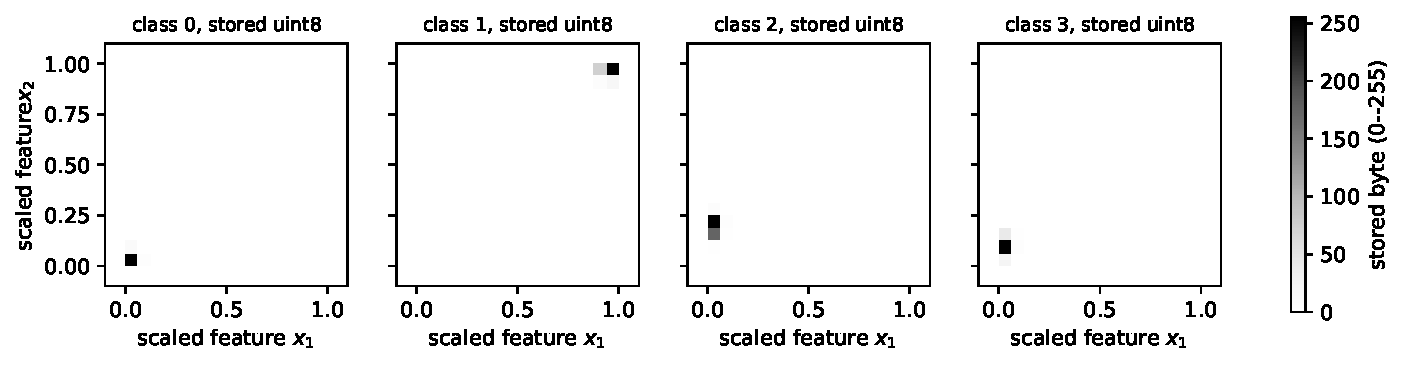
\includegraphics[width=\linewidth]{class_surfaces_discretizedLight.pdf}
    \caption{Per-class surfaces after discretization and quantization for embedded lookup.}
    \label{fig:quantized}
\end{figure}

\begin{figure}[H]
    \centering
    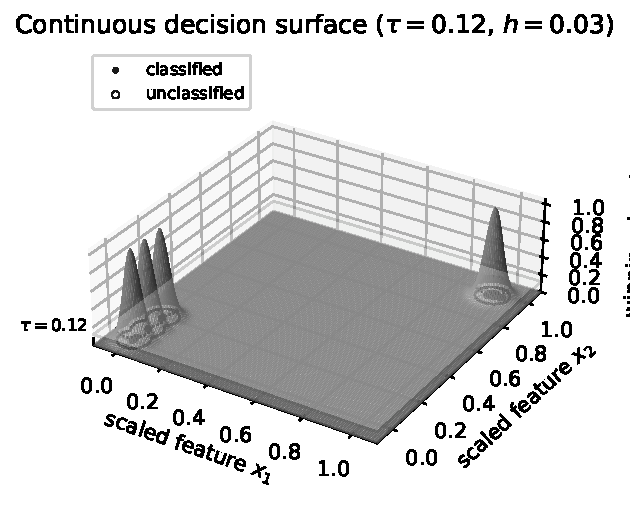
\includegraphics[width=\linewidth]{total_distributionLight.pdf}
    \caption{Combined light-classification distribution/decision surface supplied with the project.}
    \label{fig:distribution}
\end{figure}

\section{Evaluation}
\label{sec:eval}
\subsection{Desktop reference versus quantized model}
The provided confusion table compares the continuous KDE output (rows) with the stored \texttt{uint8} implementation (columns). This is an implementation-agreement test: the continuous model acts as the reference, and it does not by itself establish whether either model matches the true physical light condition.

\begin{figure}[H]
    \centering
    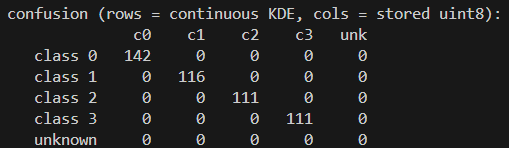
\includegraphics[width=\linewidth]{ConfusionMatrixLight.png}
    \caption{Confusion table for continuous KDE (rows) versus stored \texttt{uint8} model (columns).}
    \label{fig:confusion_image}
\end{figure}

The supplied table contains the following counts.

\begin{table}[H]
    \centering
    \caption{Continuous KDE versus quantized model.}
    \label{tab:agreement}
    \begin{tabular}{lrrrrr}
        \toprule
        Reference & C0 & C1 & C2 & C3 & Unknown\\
        \midrule
        Class 0 & 142 & 0 & 0 & 0 & 0\\
        Class 1 & 0 & 116 & 0 & 0 & 0\\
        Class 2 & 0 & 0 & 111 & 0 & 0\\
        Class 3 & 0 & 0 & 0 & 111 & 0\\
        Unknown & 0 & 0 & 0 & 0 & 0\\
        \bottomrule
    \end{tabular}
\end{table}

There are $142+116+111+111=480$ evaluated observations. All are on the diagonal, giving
\begin{equation}
    \text{agreement} = \frac{480}{480}\times100\%=100\%.
\end{equation}
No observations in this table were assigned to \emph{unknown}. The table therefore demonstrates perfect agreement on this evaluated set, but does not itself exercise the rejection option. Rejection is observed only in the device log, where 505 records are labeled \texttt{UNKNOWN} (Section~\ref{sec:stability}).


\subsection{Logged class stability}
\label{sec:stability}
The device log contains 1019 \texttt{fluorescent}, 794 \texttt{Led}, 394 \texttt{shade}, and 505 \texttt{UNKNOWN} predictions. These counts describe output labels, not the number of ground-truth samples in each class. Under the adopted rule that a label must persist for more than eight consecutive samples to count as a provisional correct/stable classification, 51 runs qualify and 26 runs do not. The heuristic is useful for flagging flicker during transitions, but a long incorrect prediction can also persist for more than eight samples; therefore it must not be described as verified accuracy.

\subsection{Scope of the accuracy claim}
The confusion table above compares two implementations of the same model rather than predictions against independently recorded ground truth, and the logged \texttt{class} column is the device's own output. Accordingly, precision, recall, F1-score, and real-world accuracy are not claimed in this report. The evidence for reliability is instead (i) implementation agreement, (ii) the signal-level filter analysis below, and (iii) temporal stability of the device output.

\subsection{Filtering evidence and signal quality}
\label{sec:filter}
Classification reliability depends on the signal the model consumes, not on agreement alone. The recording (\texttt{Assignment1.csv}) contains 2712 consecutive samples (\texttt{idx} 284--2995, no gaps) of \texttt{rawIR} and the EMA output \texttt{ir}, together with the device's predicted class. Its class column is the device's predicted output, not an independently collected ground-truth label. All four labels appear: \texttt{shade} (394 samples), \texttt{Led} (794), \texttt{fluorescent} (1019), and \texttt{UNKNOWN} (505).

\textbf{Time-domain view.} Figure~\ref{fig:rawfiltered} plots raw and filtered IR against sample index for a fluorescent-class segment; the filtered trace follows the sustained level while smoothing the sample-to-sample jitter and the short dips near samples 1282 and 1325. The first samples of the segment show the filter converging from the preceding, lower level, which is the expected EMA lag. Figure~\ref{fig:rawfilteredall} extends the view to the whole recording. Panel (a) shows that the filtered signal tracks every sustained level change between the classes (about 120, 230, 350, and above 520 counts) without flattening them, and panel (b) zooms on the largest transient: the raw value falls to about 202 counts for three samples (2785--2787) and recovers, while the filtered value bottoms out at 334 counts and stays within the same class region.

\begin{figure}[H]
    \centering
    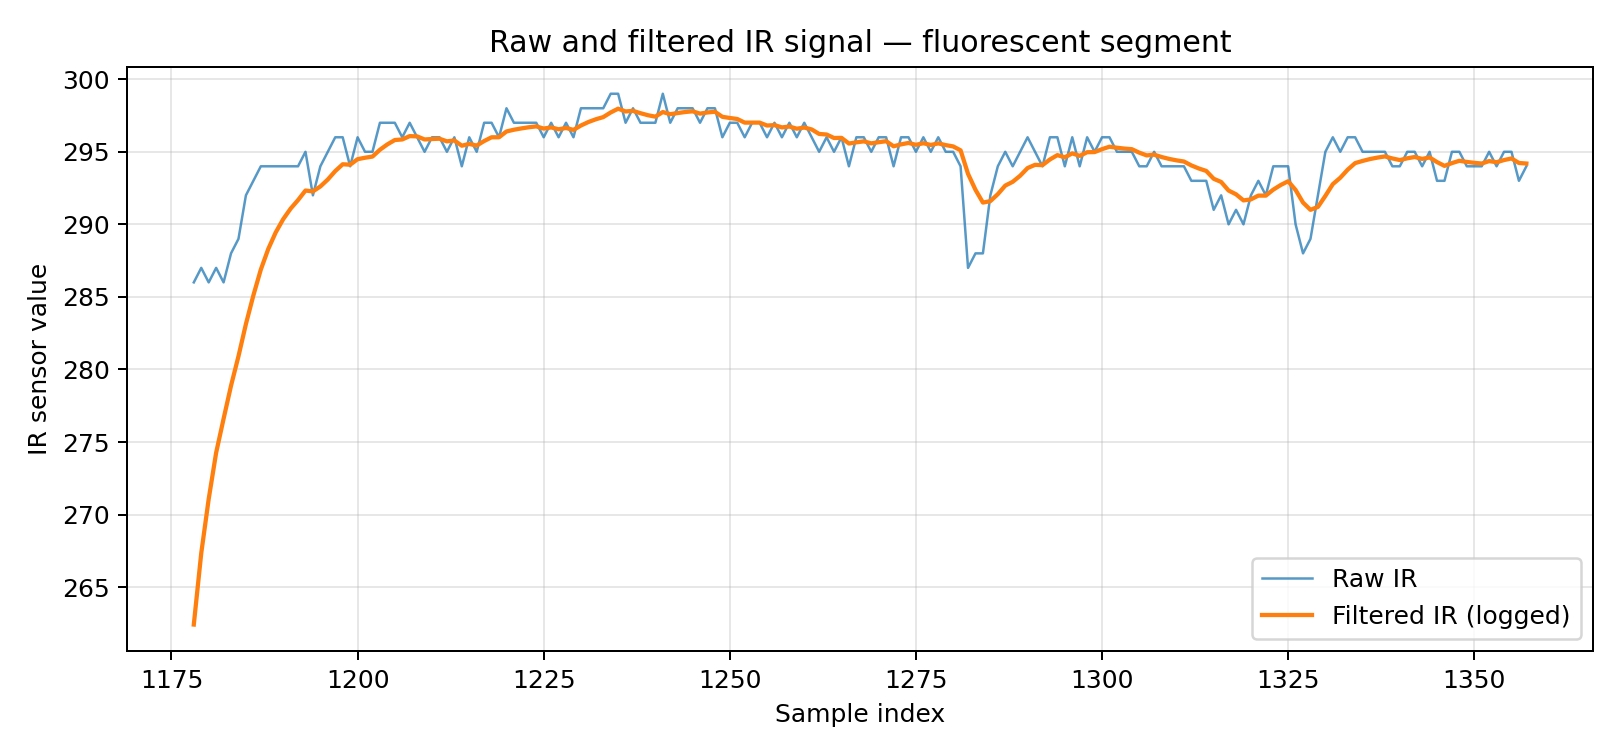
\includegraphics[width=\linewidth]{raw_vs_filtered_IR.png}
    \caption{Raw IR and logged filtered IR over a fluorescent-class segment.}
    \label{fig:rawfiltered}
\end{figure}

\begin{figure}[H]
    \centering
    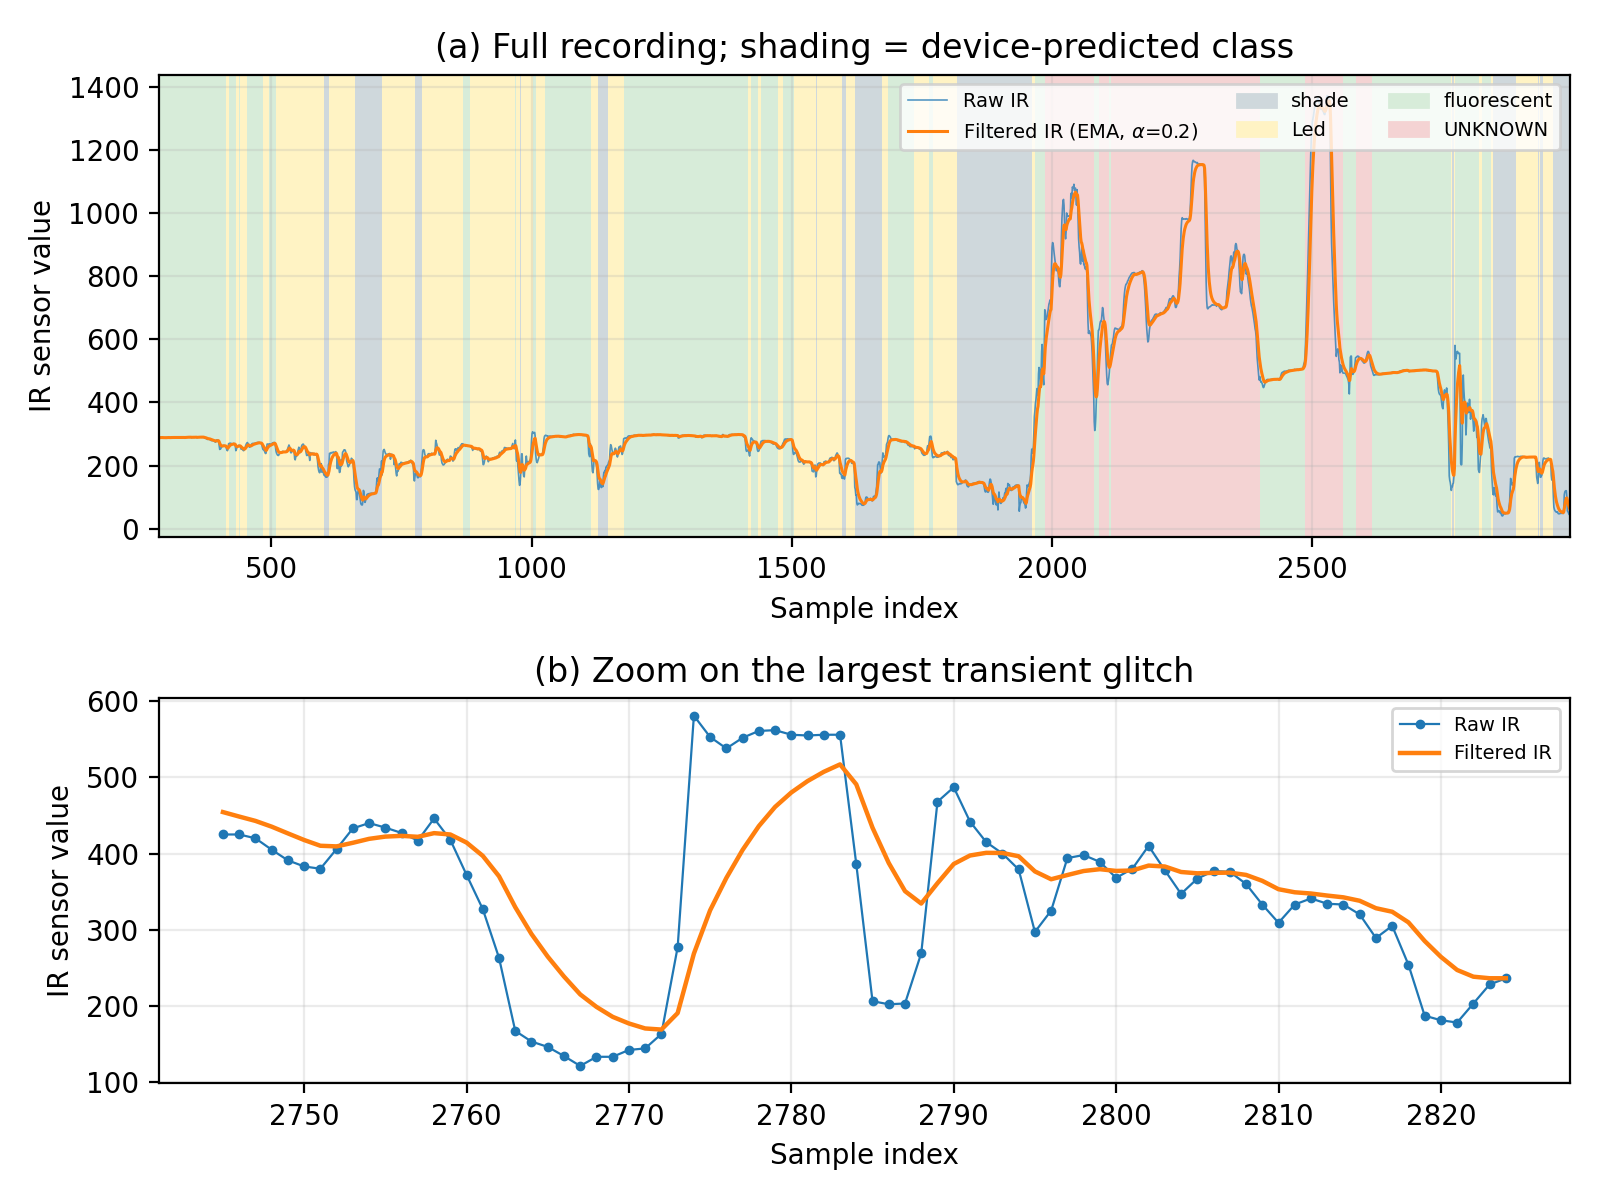
\includegraphics[width=\linewidth]{raw_vs_filtered_all_classes.png}
    \caption{(a) Raw and filtered IR over the full recording, shaded by the device-predicted class. (b) Zoom on samples 2745--2824, containing the largest transient excursion: the three-sample dip at 2785--2787 (raw about 202) is reduced to a filtered minimum of 334.}
    \label{fig:rawfilteredall}
\end{figure}

\textbf{Glitch reduction.} A transient excursion is defined as a sample whose value differs by more than 20 counts from the centered 11-sample running median of the same signal. Table~\ref{tab:filter} summarizes the effect. Raw IR has 167 such samples (largest deviation 262 counts); the filtered signal has 25 (largest deviation 63 counts), an 85\% reduction in count. The median absolute sample-to-sample step falls from 2.00 to 1.37 counts and the 95th-percentile step from 33.0 to 18.5 counts. Within every class the standard deviation of the sample-to-sample difference drops by a factor of 1.7 to 4.0 (for example, 24.1 to 6.3 counts for \texttt{fluorescent}).

\textbf{Effect on classification.} The device assigns a class from the filtered value's grid row. Applying the same row boundaries (read from the log) to \texttt{rawIR} offline, a classifier fed unfiltered data would change class 124 times instead of 76, and would produce 65 runs of eight samples or fewer instead of 26. About 9\% of samples (the 91.0\% agreement figure) would receive a different label than the one the device actually reported. This is an offline replay of the logged thresholds, not a second hardware run.

\begin{table}[H]
    \centering
    \caption{Effect of the EMA filter ($\alpha=0.2$) on the recorded IR signal.}
    \label{tab:filter}
    \footnotesize\setlength{\tabcolsep}{3pt}
    \begin{tabular}{lrr}
        \toprule
        Metric & Raw & Filtered\\
        \midrule
        Excursions $>$20 counts from median & 167 & 25\\
        Largest excursion (counts) & 262 & 63\\
        95th-pct.\ sample-to-sample step & 33.0 & 18.5\\
        Class changes (whole recording) & 124 & 76\\
        Runs of $\leq$8 samples & 65 & 26\\
        \bottomrule
    \end{tabular}
\end{table}

\textbf{Class differences are preserved.} The per-class mean levels are essentially unchanged by filtering (Table~\ref{tab:means}), so the separation between classes is not erased: the class means remain about 100 to 460 counts apart, far larger than the residual filtered jitter within a class.

\begin{table}[H]
    \centering
    \caption{Per-class mean IR value before and after filtering.}
    \label{tab:means}
    \footnotesize\setlength{\tabcolsep}{3pt}
    \begin{tabular}{lrrrr}
        \toprule
        Class & $N$ & Raw mean & Filt.\ mean & Std (raw/filt.)\\
        \midrule
        shade & 394 & 121.3 & 124.1 & 43.6 / 37.7\\
        Led & 794 & 228.9 & 229.4 & 27.0 / 19.9\\
        fluorescent & 1019 & 346.7 & 346.5 & 96.2 / 92.3\\
        UNKNOWN & 505 & 810.6 & 809.9 & 222.4 / 210.7\\
        \bottomrule
    \end{tabular}
\end{table}

\textbf{Caveats.} The EMA introduces lag: with $\alpha=0.2$ the output reaches about 90\% of a step after roughly 10 samples, so genuine transitions are reported a few samples late (visible at the start of Fig.~\ref{fig:rawfiltered}). Some of the 25 remaining excursions are genuine fast level changes rather than glitches, which the filter is not meant to remove. Because the class labels are the device's own output, the per-class statistics are descriptive rather than an independent measure of separability. Finally, \texttt{rawUV} is zero in all 2712 rows, so this recording supports only the IR channel; the pipeline's UV axis is not exercised by these data.

The recording contains \textbf{51 stable runs} (more than eight consecutive samples with the same label) and \textbf{26 short runs} under the adopted rule. This is a temporal-stability measure, not an accuracy score.

\subsection{On-device versus desktop agreement}
Agreement between the continuous KDE and the stored \texttt{uint8} tables is established by Table~\ref{tab:agreement}: 480 of 480 observations match, with no \texttt{unknown} outputs. The device log provides a consistency check of the embedded lookup itself: across all 2712 records each grid row maps to exactly one class (row 0 $\rightarrow$ \texttt{shade}, row 1 $\rightarrow$ \texttt{Led}, rows 2--3 $\rightarrow$ \texttt{fluorescent}, rows 4--6 $\rightarrow$ \texttt{UNKNOWN}), and the filtered-value ranges of the rows are contiguous and non-overlapping, as expected for a threshold-based lookup. The log does not contain the desktop model's predictions for these same samples, so a sample-by-sample desktop replay of the microcontroller log is not reported here.

\subsection{Measured prediction cost}
The table size is analytically estimated above. Prediction time was measured on the target board with a microsecond-resolution timer and logged for each of the 2712 samples (\texttt{latency\_us}); the minimum is 3~$\mu$s and the values below summarize the distribution. Compiled flash and RAM usage are taken from the build report and are not derived from the table size.

\begin{table}[H]
    \centering
    \caption{Prediction costs. Timing is taken from the supplied device log.}
    \label{tab:cost}
    \footnotesize\setlength{\tabcolsep}{3pt}
    \begin{tabular}{lll}
        \toprule
        Metric & Result & Source\\
        \midrule
        Class-table storage & 1024 bytes & Analytical estimate\\
        Scaling bounds & 16 bytes & Analytical estimate\\
        Total table + bounds & 1040 bytes & Analytical estimate\\
        Median prediction time & 6 $\mu$s & 2712 logged records\\
        Mean prediction time & 6.02 $\mu$s & 2712 logged records\\
        95th-percentile latency & 8 $\mu$s & 2712 logged records\\
        Maximum latency & 10 $\mu$s & 2712 logged records\\
        Compiled flash usage & TBD & Build report\\
        RAM usage & TBD & Build report\\
        \bottomrule
    \end{tabular}
\end{table}

Figure~\ref{fig:latency} shows the distribution of logged prediction latency. The measured median is 6~$\mu$s and the 95th percentile is 8~$\mu$s. These values describe the \texttt{latency\_us} field of the CSV, which is assumed to time the prediction call only, excluding serial output. At 6~$\mu$s the lookup is negligible next to the sensor integration time and serial printing.

\begin{figure}[H]
    \centering
    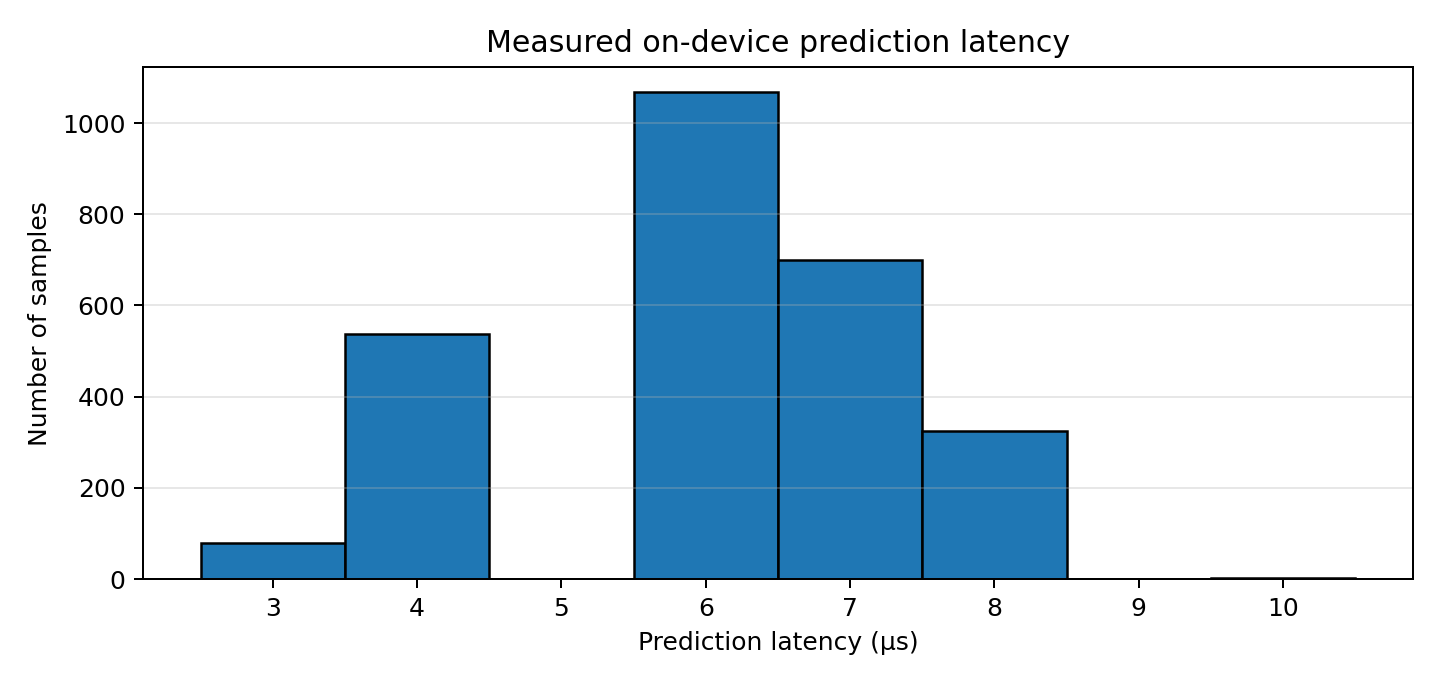
\includegraphics[width=\linewidth]{prediction_latency.png}
    \caption{Distribution of prediction latency recorded in \texttt{Assignment1.csv}.}
    \label{fig:latency}
\end{figure}

\section{Physical Proof of Concept}
Figure~\ref{fig:board} shows the wired prototype on which the log was recorded: an ESP32 development board powered over USB, an analog UV module (purple board; VCC, GND, and SIG to an ADC pin), and an Adafruit TSL2591 light sensor connected over I\textsuperscript{2}C (VIN, GND, SDA, SCL). The classifier therefore runs on the actual microcontroller with live sensor input, not only in a desktop simulation.
\begin{figure}[H]
    \centering
    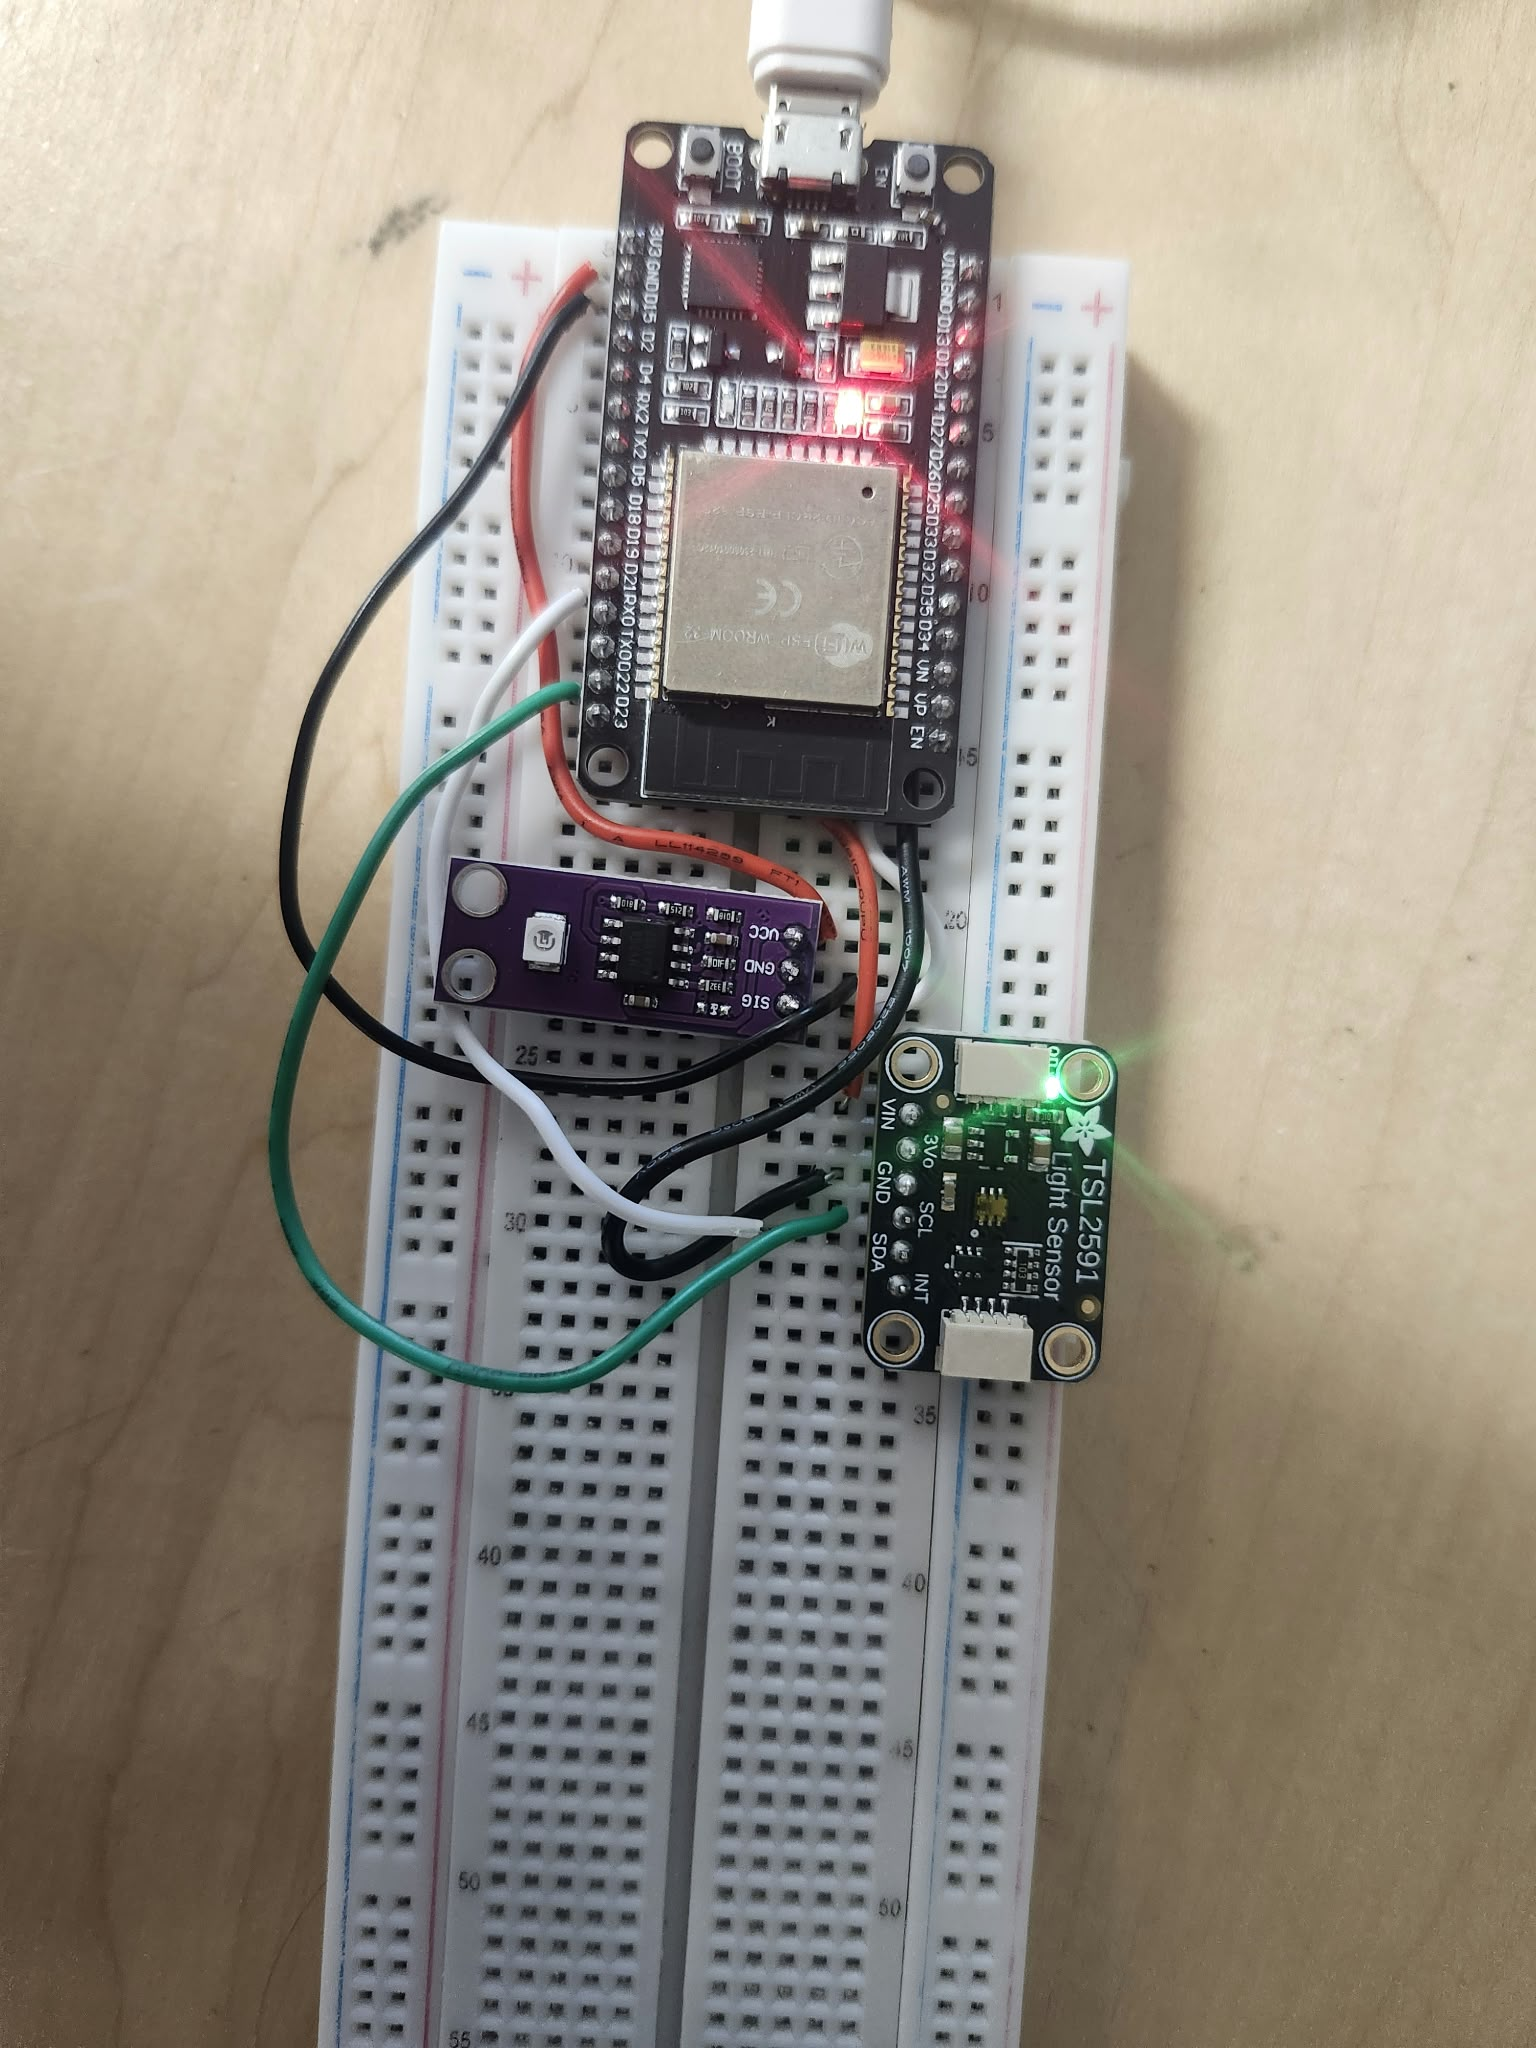
\includegraphics[width=0.6\linewidth]{BoardCircuit.png}
    \caption{Wired proof-of-concept hardware: ESP32 board, UV module, and TSL2591 light sensor.}
    \label{fig:board}
\end{figure}

\section{Limitations and Next Steps}
The evidence supports the feasibility of compressing the continuous KDE surfaces into a small lookup table and reproducing their decisions for the 480 evaluated observations, and shows that the EMA filter removes most transient excursions from the IR signal without shifting class levels. Four limitations remain. First, no independently labeled ground truth was collected, so classification accuracy is not reported. Second, the recorded UV channel is zero, so only the IR axis is evidenced in the logged data. Third, the rejection option is observed in the device log but was not tested on a dedicated out-of-distribution set. Fourth, compiled flash and RAM usage are listed as TBD in Table~\ref{tab:cost}. Natural next steps are to log labeled data per light condition, replay the logged inputs through the desktop model for a sample-by-sample comparison, and repeat the filter analysis with a working UV channel.

\section{Conclusion}
A four-class light-classification pipeline has been represented as per-class KDE surfaces and compressed into a $16\times16$ \texttt{uint8} lookup grid. The desktop comparison reports 100\% agreement over 480 observations, with 1024 bytes for class tables and 16 bytes for scaling bounds. On the 2712-sample device recording, the $\alpha=0.2$ EMA filter reduces transient excursions in the IR signal from 167 to 25 samples and spurious class changes from 124 to 76 while preserving the per-class levels, and prediction takes a median of 6~$\mu$s. Agreement between two versions of the same model is not a substitute for ground-truth testing, but together these results show that the compact classifier runs on the target hardware, consumes a cleaned signal, and is cheap enough for embedded use.

\end{document}
